\documentclass[12pt,a4paper]{article}
\usepackage[utf8]{inputenc}
\usepackage[spanish]{babel}
\usepackage{amsmath}
\usepackage{amsfonts}
\usepackage{amssymb}
\usepackage{makeidx}
\usepackage{graphicx}
\usepackage{lmodern}
\usepackage{fourier}
\usepackage[left=2cm,right=2cm,top=2cm,bottom=2cm]{geometry}
\author{Flores Macias Cesar Fabian}
\begin{document}
\begin{center}

\includegraphics[width=12cm]{Imagenes/logo.jpg}  \\
\end{center}
\textbf{UNIVERSIDAD POLITECNICA DE LA ZONA METROPOLITANA DE GUADALAJARA}\\
\textit{CONEMATICA DE ROBOTS}\\
\textit{Maestro: Carlos Enrique Moran Garabito}\\
\\ \\ \\ \\
\textit{Equipo:\\Flores Macias Cesar Fabian \\ Canales Ochoa Fabian\\ Martines Hernandes Samuel Caleb\\Gutierrez Chavez Amaury Efrain}\\
\\ \\ 
\begin{center}
Simulación de cinemática directa e inversa de manipuladores paralelo
\end{center}
. \\ \\ \textbf{Proposito:}\\
Utilizar programas de diseño y modelado en 3D para transladar el armado y la simulación al programa Gazebo, el cual es un complemento del programa ros.\\
\\
\textbf{Procedimiento:)}\\
Al tener ya listas las piezas y formato final del robot SCARA realizado y diseñado en Inventor se supondria que seria mas facil transladar todos estos datos e informacipon a un nuevo programa de diseño y modelado, Acontinuación se muestra como queda el root armado y finalizado en inventor.
\begin{center}
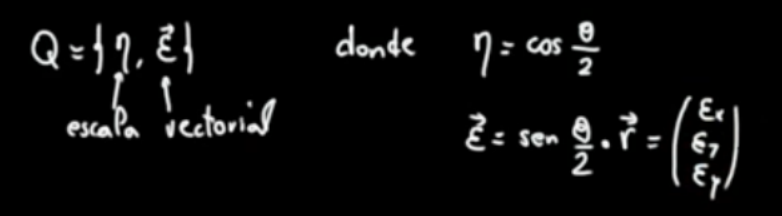
\includegraphics[width=10cm]{Imagenes/2.png}\\ Robot SCARA armado con los materiales ya definidos.
\end{center}
El programa al cual se deben transferir estos datos utiliza el formato nativo de .dae. Mientras el formato nativo de creación de inventor en .ipt.\\
\\
Esto quiere decir que debemos utilizar un programa intermido que pueda tanto leer formato .ipt y pueda exportarlo a .dae.\\
\\
Para esto se utilizo el programa llamado blender.\\
\begin{center}

\includegraphics[width=5cm]{Imagenes/B.jpeg}\\ Logotipo del programa intermediario.
\end{center}
El programa inventor puede exportar .stl el cual es leido y reproducido por blender y este a su vez puede exportar los archivos a .dae, el cual es el formato apto para Gazebo.
\begin{center}
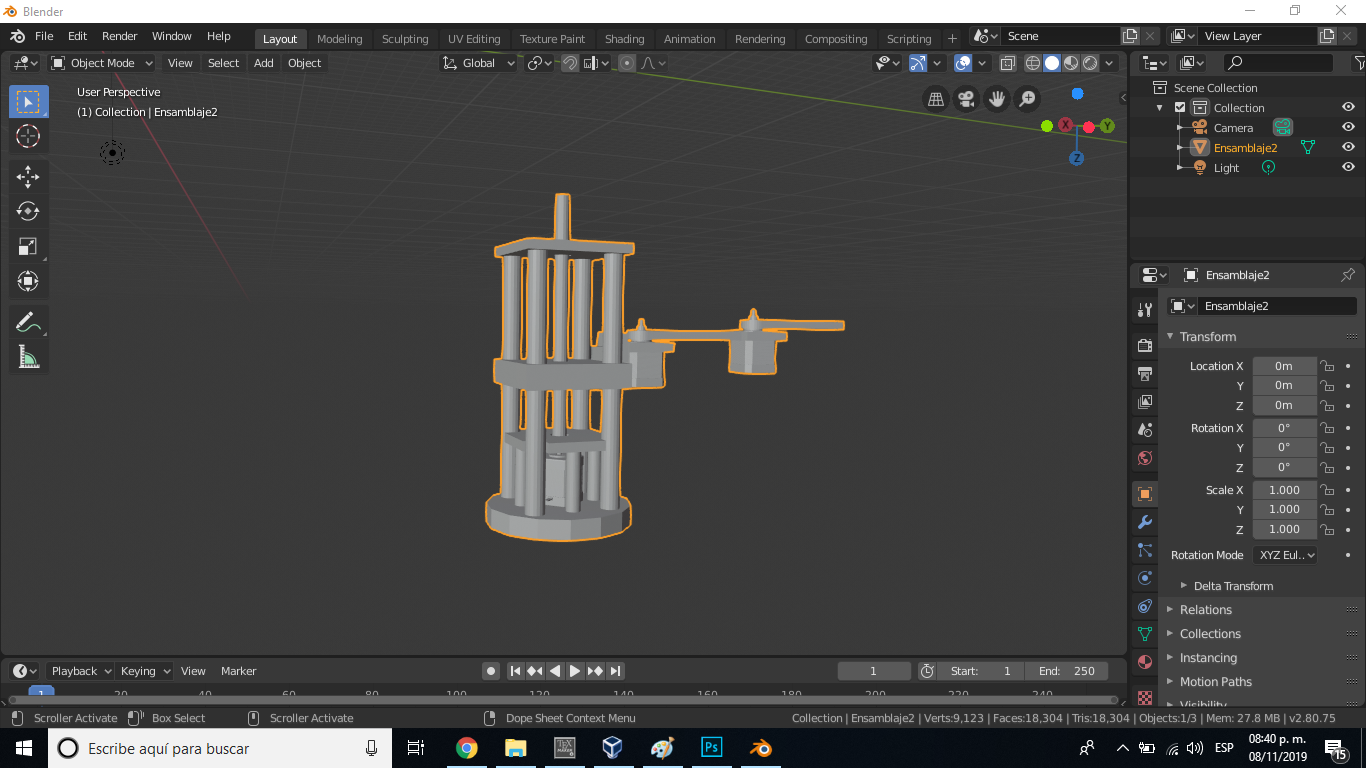
\includegraphics[width=15cm]{Imagenes/RE.png}\\ Robot en importado en Blender.
\end{center}
Al revisar este modelado en Blender pudimos aprobar la exportacioa .dae y este archivo .dae importarlo en azebo como se muestra en la siguiente imagen.\\
\begin{center}
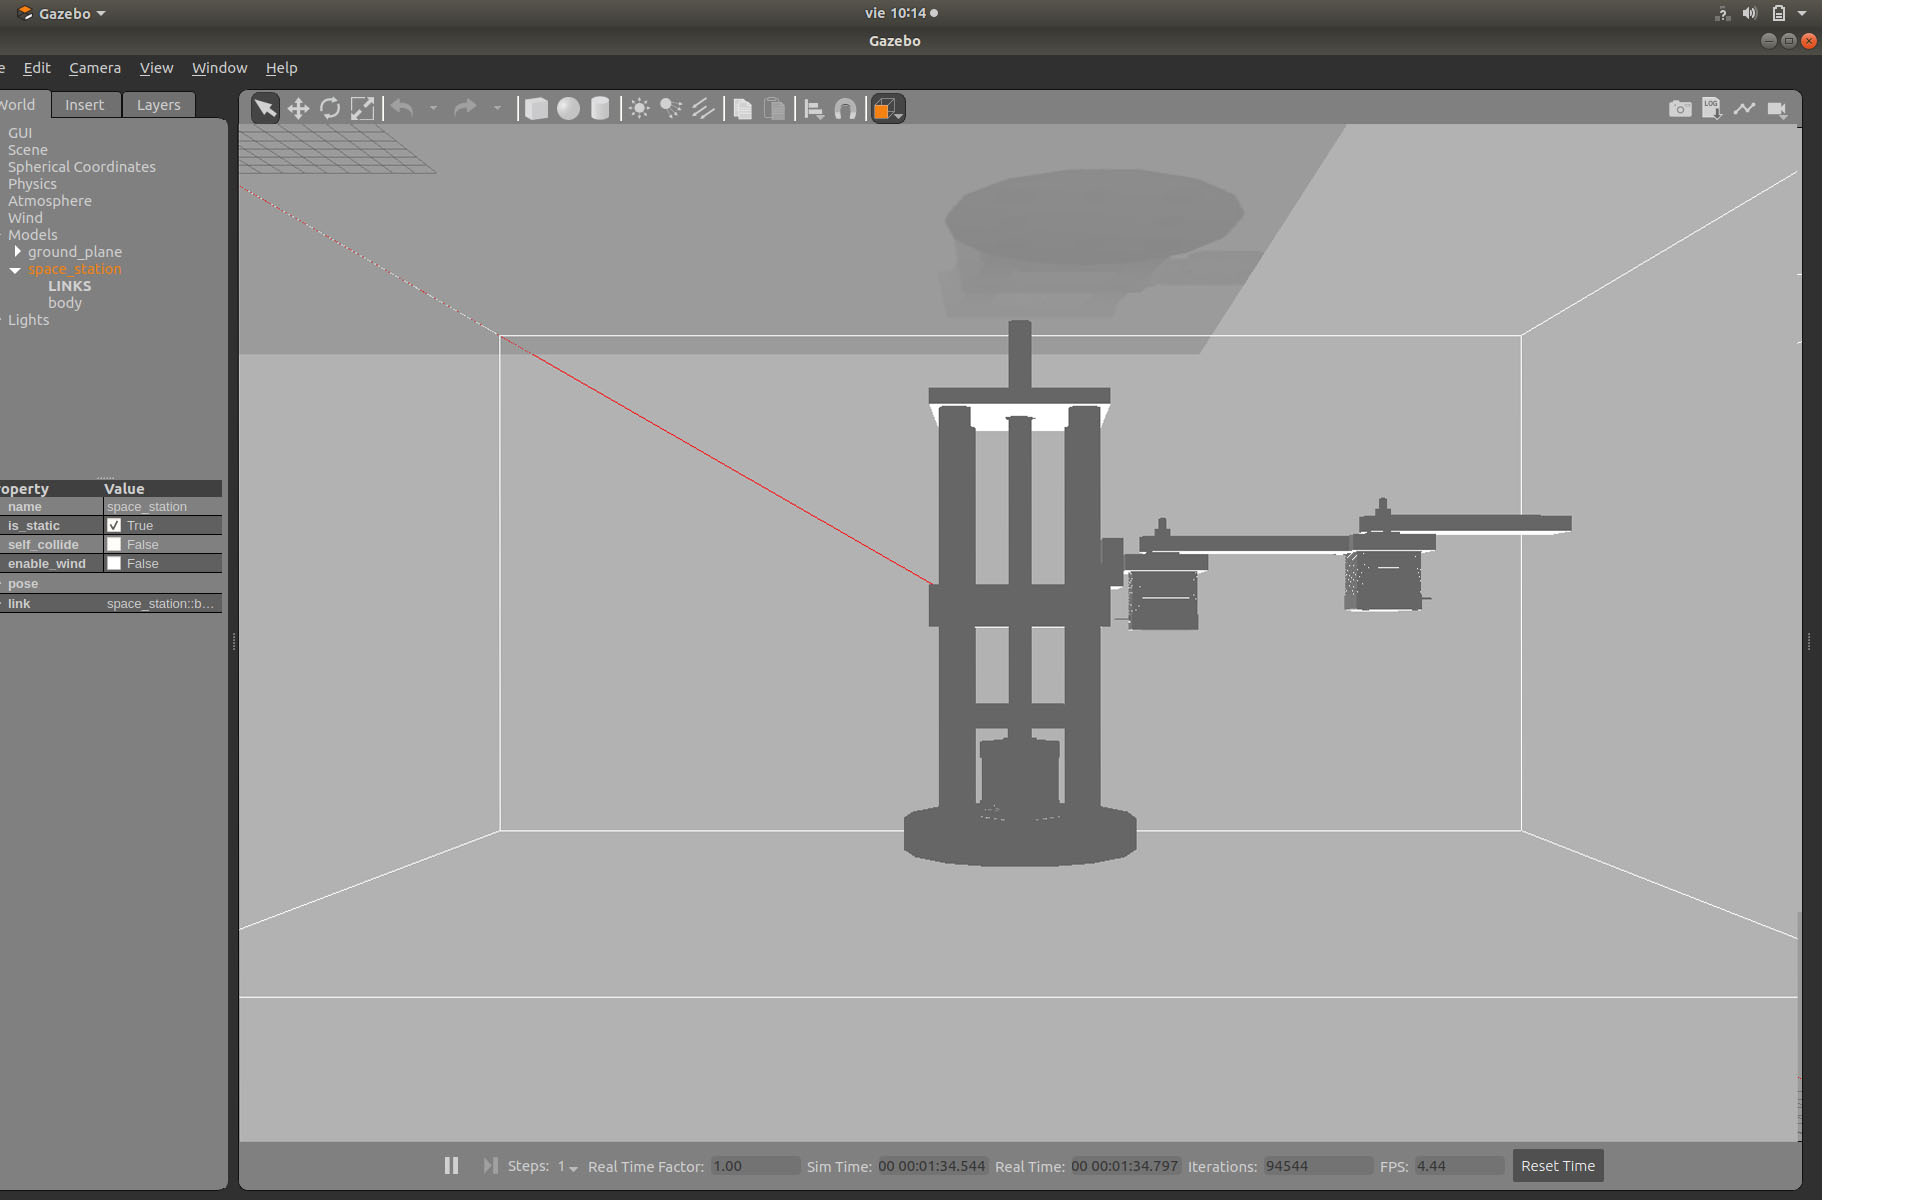
\includegraphics[width=15cm]{Imagenes/RB.jpg}\\ Robot en importado en Gazebo.
\end{center}
El importar a gazebo se debe hacer medienate comando o si al momento de instalar ROS aparece en el menu de aplicaciones de Ubuntu, al estar dentro de gazebo se debe seleccionar la pestaña "insertar" donde abrira un buscador de archivos y se debe buscar y seleccionar el archivo anteriormente importado con formado .dae.\\
\\
Si todo se realiza de manera correcta se abrira sin ningun problema, sin embargo si el archivo de gazebo no es correctamente instalado dara fallos al momento de querer abrir el archivo surgiran errores de compilación.\\
\\
\cite{koenig2004design}
\bibliographystyle{apalike} 
\bibliography{REF}
\end{document}
